\chapter{Lower bounds for depth-3 circuits over finite fields}\label{chap:GK}

This chapter shall present the lower bound of Grigoriev and Karpinski
\cite{grigoriev98} for $\SPS$ circuit computing $\Det_n$ over finite
fields. 
A follow-up paper of Grigoriev and Razborov \cite{gr00}
extended the result over function fields, also including a weaker
lower bound for the permanent, but we shall present a slightly
different proof that works for the permanent as well.

\begin{theorem}\cite{grigoriev98}\label{thm:gk-main-thm}
  Any depth-3 circuit computing $\Det_d$ (or $\Perm_d$) over a finite
  field $\F_q$ requires size $2^{\Omega_q(d)}$.
\end{theorem}

We shall also prove a similar lower bound for a version of the elementary symmetric polynomial $\ESym_d$. 

\begin{theorem}\label{thm:esym-finitefields}
  Let $n = d^2$. 
  Then, over any finite field $\F_q$, any depth-$3$ circuit computing the polynomial $\ESym_{\leq d}$ defined as
\[
\ESym_{\leq d} \spaced{\eqdef} \sum_{j\leq d} \ESym_j \spaced{=} \sum_{\substack{T \subset [n]\\ |T| \leq d}} \; \prod_{i\in T} x_i
\]
must be of size $\exp(\Omega_q(d \log n))$. 
\end{theorem}

To contrast this, over any field of at least $(n+1)$ elements, the polynomial $\ESym_{\leq d}$ can be computed by an $O(n^2)$ sized depth-$3$ circuit! This fact is attributed to Ben-Or but is a really nice exercise. 

\begin{exercise} 
Let $\F$ be a field with at least $(n+1)$ elements. 
Show that, for every $d \leq n$, there is a $\Sigma\Pi\Sigma$ 
computing  $\ESym_{d}$ of size $O(n^2)$. 

\noindent
\textcolor{gray}{\emph{Hint: } Consider $(1+tx_1) \cdots (1+tx_n)$}
\end{exercise}



{\bf Main idea:} We are working with the field $\F_q$ of $q$ elements. 
Suppose $C = T_1 + \dots + T_s$,
where each $T_i$ is a product of linear polynomials. 
Define
$\mathrm{rank}(T_i)$ as in \autoref{sec:low-rank-sps} to be the
dimension of the set of linear polynomials that $T_i$ is a product of.

In \autoref{sec:low-rank-sps}, we saw that the dimension of partial
derivatives would handle \emph{low rank} $T_i$'s. 
As for the high rank
$T_i$'s, the fact that we are working over a finite field would become
very useful. 
Since $T_i$ is a product of at least $r$ linearly
independent linear polynomials, a random evaluation keeps $T_i$
non-zero with probability at most $\inparen{1-\frac{1}{q}}^r$. 
As $q$
is a constant, we have that a random evaluation of a high rank $T_i$
is almost always zero. 
Hence, in a sense, $C$ can be ``approximated''
by just the low-rank components.

Grigoriev and Karpinski \cite{grigoriev98} formalize the above idea as
a measure by combining the partial derivative technique seen in
\autoref{sec:low-rank-sps} with evaluations to show that $\Det_d$
cannot be approximated by a low-rank $\SPS$ circuit.

\section{The complexity measure}

For any polynomial $f \in \F_q[x_{11},\dots, x_{nn}]$, define the matrix
$M_k(f)$ as follows --- the columns of $M_k(f)$ are indexed by $k$-th
order partial derivatives of $f$, and rows by elements of $\F_q^{n}$,
with the entry being the evaluation of the partial derivative (column
index) at the point (row index).\\

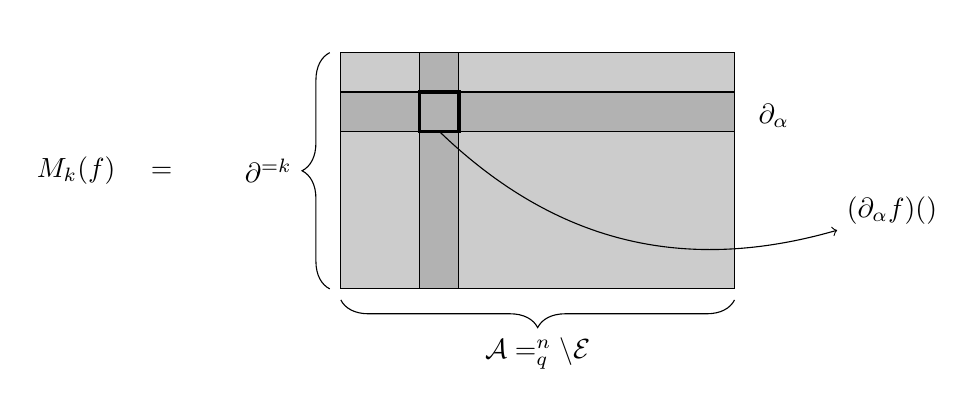
\begin{tikzpicture}
\node at (-3,1.5) {$M_k(f) \quad= $};
\draw[fill=black!20] (0,0) rectangle (5,3);

\draw[decorate,decoration={brace,amplitude=10pt,raise=4pt},yshift=0pt]
(0,0) -- (0,3);
\node[anchor=east] at (-0.5,1.5) {$\partial^{=k}$};
\draw[decorate,decoration={brace,amplitude=10pt,mirror, raise=4pt},yshift=0pt] 
(0,0) -- (5,0);
\node[anchor=north] at (2.5,-0.5) {$\mathcal{A} = \F_q^n \setminus \mathcal{E}$};

\draw[fill=black!30] (1,0) rectangle (1.5,3);
\node at (1.25,3.2) {$\veca$};

\draw[fill=black!30] (0,2) rectangle (5,2.5);
\node at (5.5,2.2) {$\partial_{\alpha}$};

\draw[very thick] (1,2) rectangle (1.5,2.5);

\node at (7,1) {$(\partial_\alpha f)(\veca)$}
edge[<-,bend left] (1.25,2);
\end{tikzpicture}


The rank of $M_k(f)$ could be a possible choice of a complexity
measure but it is not sure if $\mathrm{rank}(M_k(f))$ is small when
$f$ is even a single high rank term. 
However, Grigoriev and Karpinski
handle this by make a small modification to handle the high rank
$T_i$s. 
Instead, they look at the matrix $M_k(f)$ and remove a few
\emph{erroneous} evaluation points and use the rank of the resulting
matrix. 
For any $\mathcal{A}\subseteq \F_q^{n}$, let us define
$M_k(f;\mathcal{A})$ to be the matrix obtained from $M_k(f)$ by only
taking the rows whose indices are in $\mathcal{A}$. 
Also, let
$\CM{GK}_{k,\mathcal{A}}(f)$ denote
$\mathrm{rank}(M_k(f;\mathcal{A}))$.

\section{Upper-bounding $\CM{GK}_{k,\mathcal{A}}$ for a depth-3 circuit}\label{sec:gk-upper-bound}

Our task here is to give an upper bound on the complexity measure for
a $\SPS$-circuit of size $s$. 
We first see that the task reduces to
upper bounding the measure for a single term via subadditivity. 
It
follows from the linearity of the entries of the matrix.

\begin{observation}[Sub-additivity]\label{obs:GK-subadditivity}
  $\CM{GK}_{k,\mathcal{A}}(f + g) \quad\leq\quad
  \CM{GK}_{k,\mathcal{A}}(f) + \CM{GK}_{k,\mathcal{A}}(g)$.
\end{observation}

Let us fix a threshold $\tau$, and let $k = \tau/10q$ where $q$ is the size of the finite field we are working over.
The exact value of $\tau$ shall be fixed shortly depending on the polynomial we are proving a lower bound for. 
For $\Det_d$, we shall choose $\tau = \Omega(d)$.
For the elementary symmetric polynomial $\ESym_d$, we shall choose $\tau = \Omega(d \log n)$. 
 
We shall call a term $T = \ell_1\cdots \ell_d$ to be
of \emph{low rank} if $\mathrm{rank}(T) \leq \tau$, and \emph{large
  rank} otherwise. 
By the above observation, we need to upper-bound
the measure $\CM{GK}_{k,\mathcal{A}}$ for each term $T$, for a
suitable choice of $\mathcal{A}$.\\

\noindent 
{\bf Low rank terms $(\mathrm{rank}(T) \leq \tau)$:}

Suppose $T = \ell_1 \cdots \ell_d$ with $\inbrace{\ell_1, \dots,
  \ell_r}$ being a maximal independent set of linear polynomials (with
$r \leq \tau$). 
Then $T$ can be expressed as a linear combination of
terms from the set $\setdef{\ell_1^{e_1}\dots \ell_r^{e_r}}{e_i\leq d
  \quad \forall i\in [r]}$. 
And since the matrix $M_k(f)$ depends only
on evaluations in $\F_q^{n}$, we can use the relation that $x^q = x$
in $\F_q$ to express the evaluation of  $T$ on $\F_q^{n}$ as a linear
combination of $\setdef{\ell_1^{e_1}\dots \ell_r^{e_r}}{e_i<q \quad
  \forall i\in [r]}$. 
Therefore, for any set $\mathcal{A}\subseteq
\F^{n}$, we have that
$$
\CM{GK}_{k;\mathcal{A}}(T) \quad \leq \quad
\mathrm{rank}(M_k(f)) \quad \leq \quad q^r \quad\leq \quad q^{\tau}.
$$


\noindent
{\bf High rank terms $(\mathrm{rank}(T) > \tau)$:}

Suppose $T = \ell_1\dots \ell_d$ whose rank is greater than $\tau$, and let $\inbrace{\ell_1, \dots, \ell_r}$ be a maximal
independent set. 
We want to use the fact that since $T$ is a product
of at least $r$ independent linear polynomials, most evaluations would
be zero. 
We shall be choosing our $\mathcal{A}$ to be the set where
all $k$-th order partial derivatives evaluate to zero.

For each non-constant $\ell_i$, we know that $\Pr_{\veca} [\ell_i(\veca) = 0]  =  1/q$. 
Further, if the $\ell_i$s are linearly independent, then they \emph{independently} evaluate to zero with probability $1/q$. 
Thus, on expectation, a random point $\veca$ would evaluate to zero on $r/q > \tau/q$ of them. 
Since we chose $k = \tau/10q \ll r/q$, an application of Chernoff's bound shows that 
\[
\Pr_\veca\insquare{\text{ $\veca$ evaluates to zero on at most $k$ of the factors of $T$}} \spaced{\leq} \exp(-\tau/8)
\]
Let $\mathcal{E}_T$ be the set of $\veca$s in the above event. Then every $\veca$ outside $\mathcal{E}_T$ evaluates at least $(k+1)$ factors of $T$ to zero. 
Thus, not only is $T$ zero at $\veca$ but so are all its $k$-th order partial derivatives. 

Let $\mathcal{E}  = \Union_{T\text{ of large rank}} \mathcal{E}_T$ and let $\mathcal{A} = \F_q^n \setminus \mathcal{E}$. 
Then, for any $T\in C$ that has large rank, the matrix $M_k(T;\mathcal{A})$ is simply the zero matrix and hence $\CM{GK}_{k;\mathcal{A}}(T) = 0$. 
This means that $\CM{GK}_{k;\mathcal{A}}$ is entirely contributed by the low-rank terms. 

\begin{lemma}[Upper bound on a small circuit]\label{lem:GK-upper-bound}
Let $C$ be a depth-$3$ circuit over the field $\F_q$ of size at most $s$. Then, for any $\tau > 0$ and $k \leq \tau/10q$, there exists a set $\mathcal{E}$ of size at most $s \cdot \exp(-\tau/8) \cdot q^n$ such that 
\[
\CM{GK}_{k;\mathcal{A}}(C) \spaced{\leq} s \cdot q^{\tau}
\]
where $\mathcal{A} = \F_q^n \setminus \mathcal{E}$. 
\end{lemma}

All that is left to do now is lower bound the measure for an explicit polynomial, and set the parameter $\tau$ appropriately. We shall first consider the polynomial $\ESym_{\leq d}$ which is a little simpler, and the look at $\Det_d$ and $\Perm_d$. 

\section{Lower bound for $\Det_d$ and $\Perm_d$}

For the polynomials $\Det_d$ and $\Perm_d$, the number of variables is $n = d^2$. 
The key technical lemma is to show that
$\CM{GK}_{k,\mathcal{A}}(\Det_d)$ is large as long as
$\abs{\mathcal{A}} = (1 - o(1)) q^{d^2}$.

\begin{lemma}\label{lem:GK-technical-lemma}
  For any set $\mathcal{A} \in \F_q^{d^2}$ such that
  $\abs{\mathcal{A}} = (1 - o(1)) \cdot q^{d^2}$, we have that
  \[
  \CM{GK}_{k,\mathcal{A}}(\Det_d) \spaced{=}  \binom{d}{k}^2
  \]
\end{lemma}

The same bound shall also hold for $\Perm_d$. 
We shall defer this
theorem for later and see how this would imply the proof of
\autoref{thm:gk-main-thm}.

\begin{proofof}{\autoref{thm:gk-main-thm}}
  Let $\tau = \alpha d$, for a constant $\alpha > 0$ that shall be chosen shortly,  and $k = \tau/10q$. 
  Assume that there is a $\Sigma\Pi\Sigma$ circuit of size  $s < \exp(\tau/10) = \exp(\alpha d / 10)$ that computes $\Det_d$. 
  Then, by \autoref{lem:GK-upper-bound}, there is a set $\mathcal{A}$ of size $(1 - o(1)) q^{d^2}$ such that 
  \[
  \CM{GK}_{k;\mathcal{A}}(\Det_d) \spaced{\leq} s \cdot  q^{\alpha d}
  \]
  On the other hand, by \autoref{lem:GK-technical-lemma} we have
  \[
  \CM{GK}_{k,\mathcal{A}}(\Det_d) \spaced{=}  \binom{d}{k}^2 \spaced{=} \Omega\inparen{2^{2d \cdot H_2(\alpha/10q)}}
  \]
  where $H_2(\gamma)$ is the binary entropy function (\autoref{def:entropy}). 
  Together, this forces 
  \begin{eqnarray*}
    s \cdot q^{\alpha d}  & \geq & \Omega\inparen{2^{2d \cdot H_2(\alpha/10q)}}\\
    \implies \log s & = & \Omega((2H_2(\alpha/10q) - \alpha \log q) \cdot d)
  \end{eqnarray*}
  The binary entropy function satisfies $H_2(\epsilon) > \epsilon \log_2(1/\epsilon)$. Hence, we can always set $\alpha$ to be small enough constant to ensure that $2H_2(\alpha/10q) - \alpha \log q > 0$. 
Thus we get $s =  \exp(\Omega_q(d))$. 
\end{proofof}

\noindent
We only need to complete the proof of \autoref{lem:GK-technical-lemma}. 

\subsection{Proof of Lemma~\ref{lem:GK-technical-lemma} {} }

We now wish to show that $M_k(\Det_d;\mathcal{A})$ has large rank. 
The
original proof of Grigoriev and Karpinski is tailored specifically for
the determinant, and does not extend directly to the permanent. 
The
following argument is a proof communicated by Srikanth Srinivasan
\cite{Srikanth13} that involves an elegant trick that he attributes to
\cite{Koutis08}. 
The following proof is presented for the determinant,
but immediately extends to the permanent as well. \\


Note that if we were to just consider $M_k(\Det_d)$, it would have
been easy to show that the rank is full by looking at just those
evaluation points that keep exactly one $(d-k)\times (d-k)$ minor
non-zero (set the main diagonal of the minor to ones, and every other
entry to zero). 
Hence, $M_k(\Det_d)$ has the identity matrix
\emph{embedded inside} and hence must be full rank. 
However, we are
missing a few of the evaluations (since a small set $\mathcal{E}$ of
evaluations is removed) and we would still like to show that the
matrix continues to have full column-rank.

\begin{lemma}\label{lem:random-lc-det-nonzero}
  Let $p(X)$ be a non-zero linear combination of $r\times r$
  minors of the matrix $X = (\!(x_{ij})\!)$. 
Then, 
  $$
  \Pr_{A\in \F_q^{d^2}}[p(A) \neq 0] \quad \geq \quad \frac{q-2}{q-1}.
  $$
\end{lemma}

This immediately implies that for every linear combinations of the
columns of $M_k(\Det_d)$, a constant fraction of the coordinates have
non-zero values. 
Since we are removing merely a set $\mathcal{E}$ of
size $o(1) \cdot q^{d^2}$, there must continue to exist coordinates that
are non-zero. 
In other words, no linear combination of columns of
$M_k(\Det_d;\mathcal{A})$ results in the zero vector.


The proof of the above lemma would be an induction on the number of
minors contributing to the linear combination. 
As a base case, we
shall use a well-known fact about $\Det_d$ and $\Perm_d$ of random
matrices.

\begin{proposition}\label{prop:random-det-nonzero}
  If $A$ is a random $d\times d$ matrix with entries from a fixed
  finite field $\F_q$, 
$$
\Pr[\det(A) \neq 0] \quad\geq\quad \frac{q-2}{q-1}.
$$
\end{proposition}

The proof of this is in fact a nice exercise, and we give a few hints
at the end of this section. 
Let us begin with the proof of
\autoref{lem:random-lc-det-nonzero}.

\begin{proof}[Proof of \autoref{lem:random-lc-det-nonzero}]
  If $p(X)$ is a scalar multiple of a single non-zero minor, then we
  already have the lemma from
  \autoref{prop:random-det-nonzero}. 
Hence, let us assume that
  there are at least two distinct minors participating in the linear
  combination $p(X)$. 
Without loss of generality, assume that the
  first row occurs in some of the minors, and does not in others. 
That is, 
  \begin{eqnarray*}
    p(X) &=& \inparen{\sum_{i:\text{Row}_1\in M_i} c_i M_i} \quad+ \quad \inparen{\sum_{j:\text{Row}_1\notin M_j} c_j M_j}\\
     & = & \inparen{x_{11} M_1' + \dots + x_{1d} M_{d}'} \quad+\quad M'' \quad\text{(expanding along the first row)}.
  \end{eqnarray*}
  
  To understand a random evaluation of $p(X)$, let us first set rows
  $2, \dots, d$ to random values, and then setting row $1$ to random
  values.
  \begin{eqnarray*}
    \Pr_{A}[p(A)\neq 0] & \geq & \Pr[x_{11} M_1' + \dots + x_{1d} M_d' + M'' \neq 0 \;|\; \text{some }M_{i}'\neq 0]\\
    & & \quad \times \Pr[\text{some }M_i' \neq 0]
  \end{eqnarray*}
  Note that once we have set rows $2,\dots, d$ to random values,
  $p(X)$ reduces to a linear polynomial in $\inbrace{x_{11},\dots,
    x_{1d}}$. 
Further, a random evaluation of any non-constant linear
  polynomial is zero with probability exactly $\inparen{1
    -\frac{1}{q}}$. 
Hence,
  \begin{eqnarray*}
\Pr_{A}[p(A)\neq 0] & \geq & \Pr[x_{11} M_1' + \dots + x_{1d} M_d' + M'' \neq 0 \;|\; \text{some }M_{i}'\neq 0]\\
 & & \quad \times \Pr[\text{some }M_i' \neq 0]\\
    & = & \inparen{1 - \frac{1}{q}}\cdot \Pr[\text{some }M_i' \neq 0].
  \end{eqnarray*}
  Now comes  Koutis' Trick: the term $\inparen{1 -
    \frac{1}{q}} \cdot \Pr[\text{some }M_i' \neq 0]$ is exactly the
  probability that $x_{11}M_1' + \dots + x_{1d}M_d'$ is non-zero! 
Hence,
\begin{eqnarray*}
\Pr_{A}[p(A) \neq 0] & = & \Pr[ x_{11}M_1' + \dots + x_{1d} M_d' + M''\neq 0]\\
 & \geq & \Pr[ x_{11}M_1' + \dots + x_{1d} M_d'\neq 0]\\
 & = & \Pr\insquare{\inparen{\sum_{i:\text{Row}_1\in M_i} c_i M_i} \neq 0}.
\end{eqnarray*}
which is just the linear combination obtained by only considering
those minors that contain the first row. 
Repeating this process for other
rows/columns until only  one minor remains, we have
$$
\Pr_{A}[p(A) \neq 0] \quad \geq \quad \Pr_{A}[\det(A) \neq 0] \quad = \quad
\frac{q-2}{q-1}\quad(\text{by \autoref{prop:random-det-nonzero}}).\qedhere
$$
\end{proof}


\begin{exercise}[Proving \autoref{prop:random-det-nonzero}]
  Let $\inbrace{q_n}$ be a sequence of non-negative reals such that $\sum q_n$ converges to some $s < 1$. 
Show that 
  \[
  \prod_{i=1}^{\infty} (1 - q_n) \quad \geq \quad 1 - s. 
  \]
  Use this to infer that the probability that a random $n\times n$ matrix $A$ over $\F_q$ is invertible, which is exactly
  \[
  \inparen{1 - \frac{1}{q}}\cdots \inparen{1 - \frac{1}{q^{n}}},
  \]
  is at least $1/4$. 
\end{exercise}

\begin{exercise}[Proving \autoref{prop:random-det-nonzero} for $\Perm_n$]
  Show that
  \begin{eqnarray*}
    \Pr_{A \in \F_q^{n\times n}}[\Perm(A) = 0] & \leq &  \frac{1}{q^n} + \frac{1}{q^{n-1}} + \cdots + \frac{1}{q}\\
    & = & \frac{1}{q-1}\inparen{1-\frac{1}{q^n}}.
  \end{eqnarray*}
  \textcolor{gray}{Hint: Use Koutis' trick (\autoref{lem:random-lc-det-nonzero}).}
\end{exercise}

\section{Lower bound for $\ESym_{\leq d}$}

The goal of this section would be to get a lower bound on $\CM{GK}_{k;\mathcal{A}}(\ESym_{\leq d})$, where $n = d^2$, when $k$ is suitably chosen. In this case, we shall set $\tau = \alpha \cdot d \log n$ for a constant $\alpha>0$ that shall be chosen shortly, and $k = d/2$. The main lemma of this section would be the following. 

\begin{lemma}\label{lem:esym-d3measure-lb}
Consider the polynomial $\ESym_{\leq d}$ with $n = d^2$. If $k = d/2$ and $\mathcal{A} = \F_q^n \setminus \mathcal{E}$ with $\abs{\mathcal{E}} \leq \exp(-\omega(d\log q)) \cdot  q^n$, then
\[
\CM{GK}_{k;\mathcal{A}}(\ESym_{\leq d}) \spaced{\geq} \binom{n}{d/2}
\]
\end{lemma}

\noindent
We shall prove this lemma shortly but let us first see how this implies \autoref{thm:esym-finitefields}. 

\begin{proof}[Proof of \autoref{thm:esym-finitefields}]
Assume that the polynomial $\ESym_{\leq d}$ can be computed by a $\Sigma\Pi\Sigma$ circuit of size $s \leq \exp(\tau/10) = \exp((\alpha/10) \cdot d \log n)$. Then, by \autoref{lem:GK-upper-bound}, there is a set $\mathcal{E}$ with $\abs{\mathcal{E}} \leq \exp(-\Omega(d\log n)) \cdot q^n \ll \exp(-\omega(d \log q)) \cdot q^n$ such that
\[
\CM{GK}_{k;\mathcal{A}}(\ESym_{\leq d}) \spaced{\leq} s \cdot q^{\alpha\cdot d\log n}
\]
where $k = d/2$ and $\mathcal{A} = F_q^n \setminus \mathcal{E}$. On the other hand, from \autoref{lem:esym-d3measure-lb} we get
\[
\CM{GK}_{k;\mathcal{A}}(\ESym_{\leq d}) \spaced{\geq} \binom{n}{d/2} \spaced{\geq} 2^{(d/4) \log d}
\]
These two bounds force $s \geq \exp(\Omega_q(d \log d)) = \exp(\Omega_q(d\log n))$. 
\end{proof}

\noindent
We only need to prove \autoref{lem:esym-d3measure-lb} to complete the proof. 

\subsection{Proof of Lemma~\ref{lem:esym-d3measure-lb}}

We have set $k = d/2$ and are hence studying the evaluations partial derivatives of $\ESym_{\leq d}$ of order $d/2$ on points in $\mathcal{A}$. Let us first focus on the partial derivatives as formal polynomials. \\

Consider the following matrix $M$ where each rows is indexed by a partial derivative of order $k = d/2$, columns indexed by monomials of degree $d -d/2 = d/2$ and the corresponding entry being $1$ if that monomial occurs in partial derivative of $\ESym_{\leq d}$ and zero otherwise. That is, each row of this matrix is a partial derivative of $\ESym_{\leq d}$ written down via its coefficients. Now notice that if we have a partial derivative corresponding to a subset $S$, a monomial corresponding to a subset $T$ would be present in $\partial_S(\ESym_{\leq d})$ if and only if $|T| \leq d/2$ and $S \intersection T = \emptyset$. These $\binom{n}{d/2} \times \binom{n}{\leq d/2}$ matrices have been well studied and are called  \emph{Disjointness Matrices}. The following lemma of Razborov~\cite{razborov87} shows that these matrices are full-rank. 
\begin{lemmawp}[Rank of disjointness matrices \cite{razborov87}] Let $D$ be a $\binom{n}{d} \times \binom{n}{\leq d}$ matrix such that 
\[
D(S,T) \spaced{=} \begin{cases}
  1 & \text{if $S \intersection T = \emptyset$}\\
  0 & \text{otherwise}
\end{cases}
\]
Then, over any field $\F$, the matrix $D$ has rank $\binom{n}{d}$. 
\end{lemmawp}

Thus stated differently, this says that the $(d/2)$-th partial derivatives of $\ESym_{\leq d}$ are linearly independent as formal polynomials over any field $\F$. We would like to use this to infer that the matrix $M_k(f;\mathcal{A})$ is also full-rank as long as $\mathcal{A} = \F_q^n \setminus \mathcal{E}$ and $|\mathcal{E}| \leq \exp(-\omega(d \log q)) \cdot q^n$. 

Consider any linear combination of $(d/2)$-th order partial derivatives of $\ESym_{\leq d}$. We know that this is a non-zero multilinear polynomial of degree $d/2$. The following exercise shows that non-zero multilinear polynomials of low-degree must have many non-zero evaluations. 

\begin{exercise}[Schwartz-Zippel over small fields]
Show that, over any field $\F_q$, any non-zero multilinear $n$-variate  polynomial $f$ of degree $d$ evaluates to a non-zero value on at least $q^{n-d}$ points of $\F_q^n$. 
\end{exercise}

Thus, any linear combination of partial derivatives must be non-zero on at least $q^{-d/2} \cdot q^n = \exp(-(d/2) \log q) \cdot q^n$ points. Since $|\mathcal{E}| < \exp(-\omega(d \log q) \cdot q^n$, we cannot have thrown away all the non-zero evaluations. Thus, for every linear combination of partial derivatives, there must exist some point $\veca \in \mathcal{A}$ on which it evaluates to a non-zero value. In other words, no linear combination of rows of $M_k(\ESym_{\leq d};\mathcal{A})$ yields the zero row and hence is full rank. \qed


%%% Local Variables: 
%%% mode: latex
%%% TeX-master: "fancymain"
%%% End: 
